
\section{Summative Evaluation}
\label{sec:summative-evaluation}

Phase D of the project (June 2011 – February 2012, see Section 3)
included summative evaluation of the TA tools. This evaluation
comprised two parts. The first part was a classroom-based trial
involving one of our teacher collaborators at her school.  This
teacher had worked closely with us in Phase A and indeed was one of
the teachers who had participated in a classroom trial in Phase B. A
one-to-one session was first held with this teacher where she was
introduced to the final versions of the TA tools, and where she
planned two one-hour lessons that she would undertake with a class of
28 14-year olds using the MiGen system. During the first lesson, the
TA tools were installed on a tablet PC which she carried around the
class with her and consulted as she wished as her students were
undertaking the task set in eXpresser. During the second lesson, which
took place the next day, the teacher did not have access to the TA
tools and had to support the students as they were working with
eXpresser without having access to the information that the TA tools
provide.  During and at the end of both lessons a member of the
research team “shadowed” the teacher and asked her a number of
questions covering between them all the usage scenarios US1-US8, with
the aim of finding out the extent to which the TA tools met the
requirements of the usage scenarios. These questions are listed in
Appendix\ref{rrk}. 
 
*** Analysis of the two sets of responses to the questions is needed
here ****


The second part of the summative evaluation involved a 2-hour session
held with a new cohort of 11 trainee maths teachers on the
Postgraduate Certificate in Education programme at the IoE. Each of
the participants had an installation of the MiGen system running on
their computer. In the first half of the session, participants were
introduced to the MiGen project, the MiGen system as a whole, the
eXpresser, and the TA tools. In particular, the TA tools were
introduced to participants loaded with the real student interaction
data as arising from the classroom trial undertaken in the first part
of the summative evaluation and described above. Participants were
then asked to use the TA tools and the time-stop functionality to
answer a short list of questions relating to usage scenarios US1-US6
at different time points in the lesson. The questions are listed in
Appendix 2 (each relating to a usage scenario). 
Participants were also asked how long it would take them to
answer these questions in the classroom – our aim being not only to
determine if participants were able to use the TA tools to answer the
questions correctly, but how they perceived the amount of time it
would take them to answer the questions in a classroom situation. 

\begin{table}[tb]
  \centering
  \begin{framed}
  \begin{itemize}
  \item Q1. The session started~10’~ago (“10~minutes on”). If you chose a
    student to help immediately, which student(s) would you choose and
    why?
  \item Q2. Based on your experience and previous sessions you would have
    expected by now (“10~minutes on”) that students have achieved at
    least two goals. With a quick glance of the tools would you say
    that the class overall is going according to plan or would you
    intervene and why?
  \item Q3. We are at “30~minutes on”. Based on your experience and
    previous sessions you expected that students would have finished
    by now so that you can progress on the next task. With a quick
    glance of the tools do you think that the class is at that stage
    and why?
  \item Q4. Sometimes students are off-task (e.g. play
    games). At~“30~minutes on”, find two students that are
    disengaged/distracted?
  \item Q5. We are at~“30~minutes on”. Some students need help and you are
    trying to identify others who have finished and can help them. Can
    you give two examples of students who have finished? 
  \end{itemize}    
  \end{framed}
  \vspace{-1em}
  \caption{Questions asked to trainee Math teachers for the summative
    evaluation of the Teacher Assistance tools. Teachers had to answer
    the question and record the time they needed to do so (ranging
    from ``1 -- Very little'' to ``5 -- A lot of time'')} 
  \label{fig:questions-pgce}
\end{table}

All students provided correct examples without any assistance from the
team. The graph shown in Figure~\ref{fig:perceived-time} analyses the
responses relating to the perceived length of time required to
 answer each question. We see, that for all
the questions, no participant responded that they needed a long time
or a lot of time to answer. The questions that were regarded as
requiring the least time to answer were questions 1, 4 and 5, most
likely because they pertain to individual students and could be
answered by consulting just a single tool (the CD tool). Questions 2
and 3 may have appeared to participants as taking more time to answer
because they refer to the classroom as a whole and because, in order
to have a better picture, participants may have consulted the GA tool
as well, and even the ST tool in Question 2 for a more detailed view
of how students are progressing with their constructions. On the
whole, we consider the responses satisfactory particularly as no
answers were perceived as requiring long or a lot of time, which was
our aim. 

\begin{figure}[htbp]
  \centering
    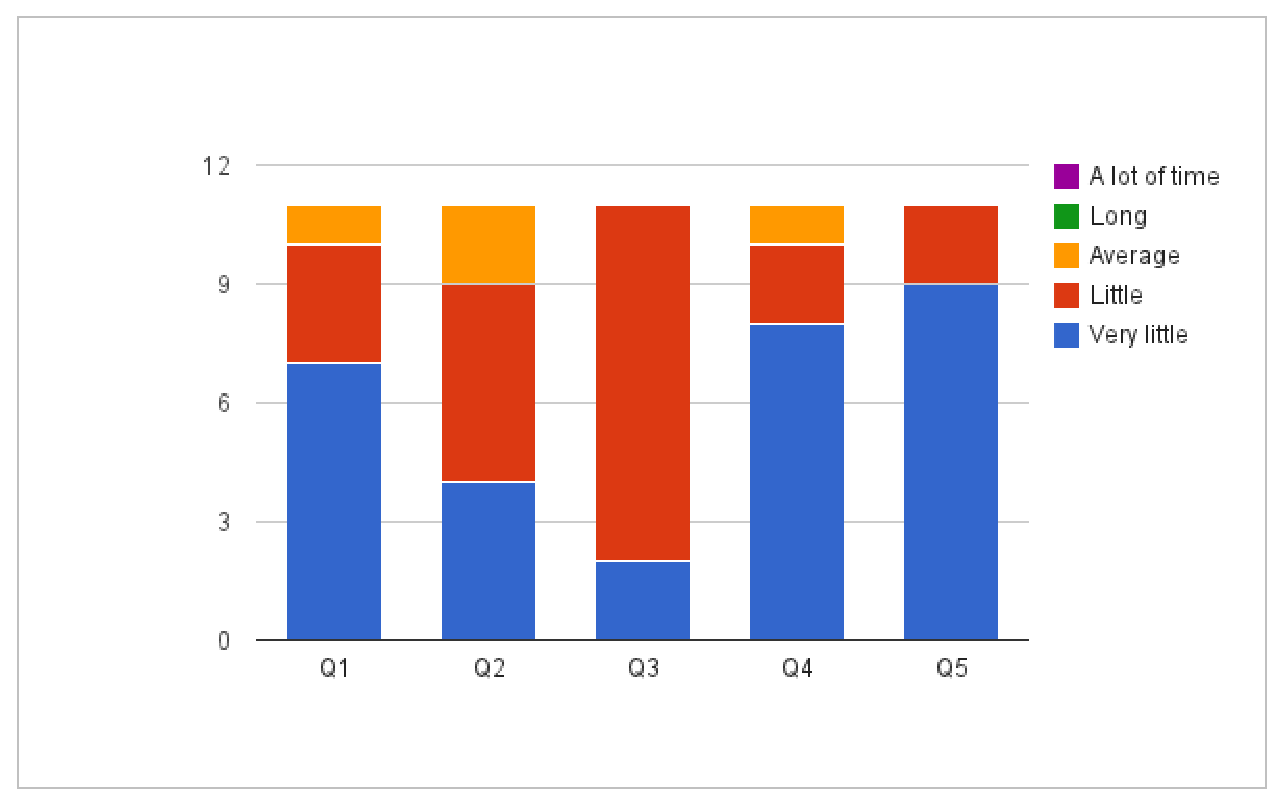
\includegraphics[width=\textwidth]{gfx/perceived-time-Q1-Q5.eps}
  \caption{Participants' perceived time to answer the questions in
Table~\ref{fig:questions-pgce}} 
\label{fig:perceived-time}
\end{figure}


Finally, participants were asked to respond to the following list of
questions, relating to their perceived usefulness of the TA tools for
usage scenarios US1-US8 (where Q1 relates to US1, Q2 to US3, Q3 to
US6, Q4 to US2 and US7(i), Q5 to US7(ii), Q6 to US8, Q7 to US4.) Their
response to each question was selected from 5 choices: Totally Agree,
Agree, Not sure, Disagree, Totally Disagree.

\begin{figure}[htbp]
  \begin{framed}
  I think that the Teacher Assistance Tools (TAT) can help me\ldots
  \begin{enumerate}
  \item \ldots in the
    classroom to find out which students need the teacher's immediate
    help.
  \item \ldots in the classroom to find out which students are
    currently disengaged from the task or distracted.
  \item \ldots to identify which goals have been achieved by which
    students.
  \item \ldots to provide appropriate support and guidance to individual
    students during the lesson.
  \item \ldots to provide appropriate support and guidance to individual
    students and reflect on the class' progress after the lesson.
  \item \ldots to reflect on the class' achievements and to plan for
    the next lesson.
  \item either in the classroom or after the class, to identify common
    conceptual and procedural difficulties students are facing in
    order to prove more explanation to the class as a whole in the
    current or the next session.
  \end{enumerate}
  \end{framed}
  \vspace{-1em}
  \caption{Additional questions asked to trainee Math teachers for the
    summative evaluation of the Teacher Assistance tools (answers
    ranging from ``1 -- Totally Disagree'' to ``5 -- Totally Agree'')} 
  \label{fig:questions2-pgce}    
\end{figure}



\begin{figure}[htbp]
  \centering
    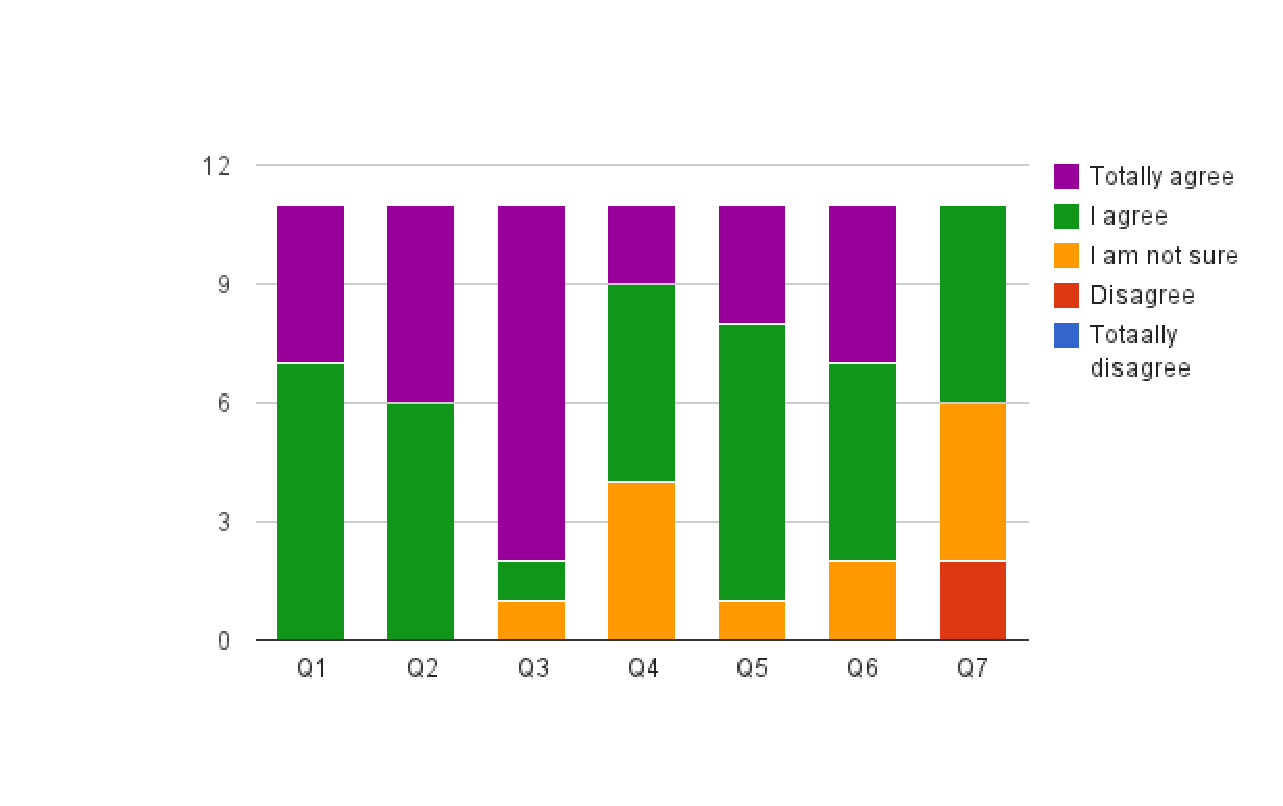
\includegraphics[width=\textwidth]{gfx/agreement.eps}
  \caption{Agreement to the statements in Table~\ref{fig:questions2-pgce}} 
\label{fig:additional}
\end{figure}

Figure~\ref{fig:perceived-time} presents the responses relating to each
question. We 
see that there are no responses of Totally Disagree to any question,
and that only Q7 attracted 2 answers of Disagree. Q1, Q2, Q3, Q5, Q6
had mostly responses of Agree or Totally Agree. Q4 had 4 responses of
Not Sure, and it related to using the tools to inform the provision of
support and guidance to students during the lesson. Q7 had the worst
pattern of responses, with 2 answers of Disagree and 4 answers of Not
Sure, and it related to identifying common conceptual or procedural
difficulties that students are facing. We discuss these results in
more detail in the next Section.




%%% Local Variables:
%%% mode: latex
%%% TeX-master: "main"
%%% End:
